\section{\tttfull (\ttt)}
\label{appendix:ttt-plot}

\begin{figure}[H]
    \centering
    \begin{subfigure}{0.49\textwidth}
        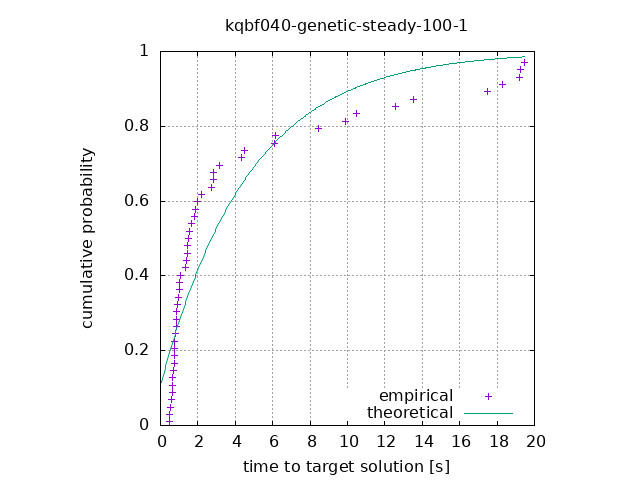
\includegraphics[width=\textwidth]{figure/ttt_plot/kqbf040-genetic-steady-100-1-exp.jpeg}
        \caption{Cumulative Probability Distribution - Algorithm GA steady - Problem kqbf040}
        \label{fig:ga-steady-kqbf040-exp}
    \end{subfigure}
    \hfill
    \begin{subfigure}{0.49\textwidth}
        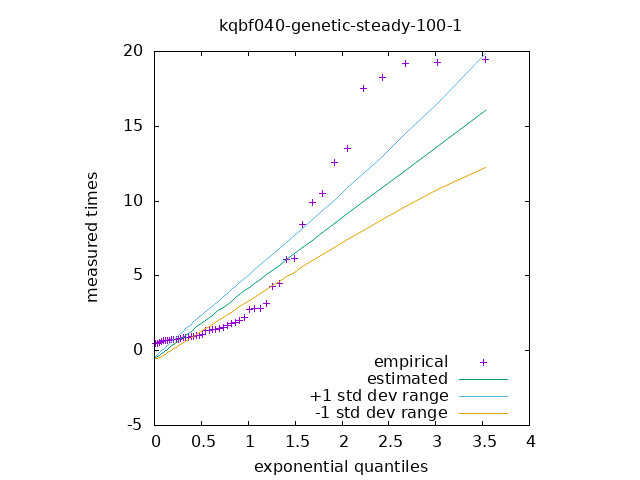
\includegraphics[width=\textwidth]{figure/ttt_plot/kqbf040-genetic-steady-100-1-qq.jpeg}
        \caption{Q-Q plot - Algorithm GA steady - Problem kqbf040}
        \label{fig:ga-steady-kqbf040-qq}
    \end{subfigure}
    \caption{Algorithm GA steady - Problem kqbf040.}
    \label{fig:ga-steady-kqbf040}
\end{figure}


\begin{figure}[H]
    \centering
    \begin{subfigure}{0.49\textwidth}
        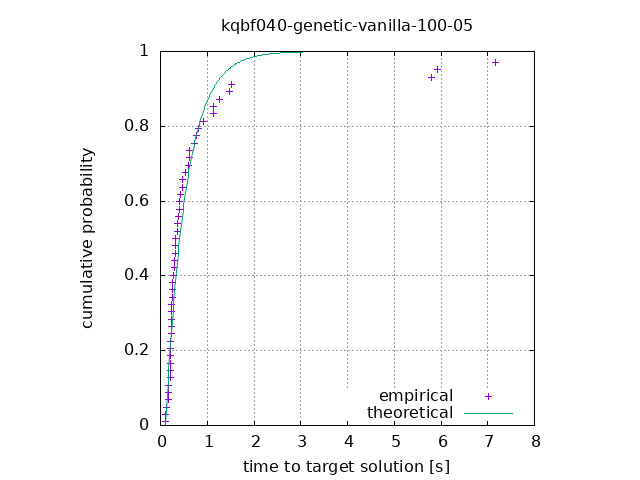
\includegraphics[width=\textwidth]{figure/ttt_plot/kqbf040-genetic-vanilla-100-05-exp.jpeg}
        \caption{Cumulative Probability Distribution - Algorithm GA vanilla - Problem kqbf040}
        \label{fig:ga-vanilla-kqbf040-exp}
    \end{subfigure}
    \hfill
    \begin{subfigure}{0.49\textwidth}
        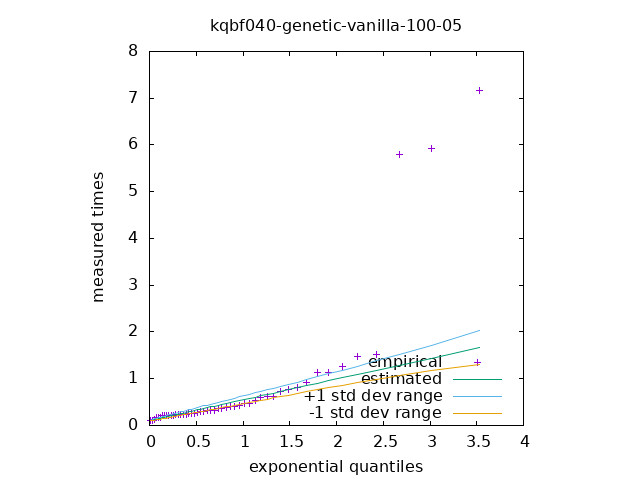
\includegraphics[width=\textwidth]{figure/ttt_plot/kqbf040-genetic-vanilla-100-05-qq.jpeg}
        \caption{Q-Q plot - Algorithm GA vanilla - Problem kqbf040}
        \label{fig:ga-vanilla-kqbf040-qq}
    \end{subfigure}
    \caption{Algorithm GA vanilla - Problem kqbf040.}
    \label{fig:ga-vanilla-kqbf040}
\end{figure}


\begin{figure}[H]
    \centering
    \begin{subfigure}{0.49\textwidth}
        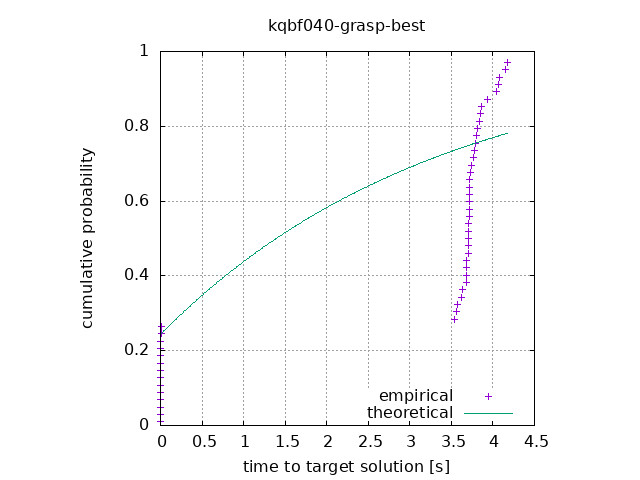
\includegraphics[width=\textwidth]{figure/ttt_plot/kqbf040-grasp-best-exp.jpeg}
        \caption{Cumulative Probability Distribution - Algorithm GRASP Best - Problem kqbf040}
        \label{fig:grasp-best-kqbf040-exp}
    \end{subfigure}
    \hfill
    \begin{subfigure}{0.49\textwidth}
        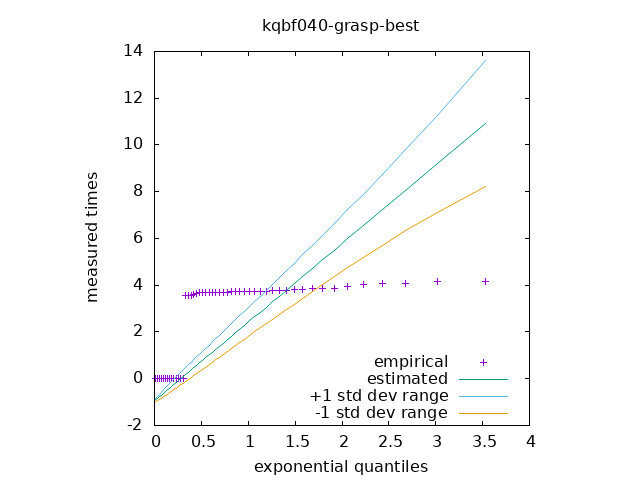
\includegraphics[width=\textwidth]{figure/ttt_plot/kqbf040-grasp-best-qq.jpeg}
        \caption{Q-Q plot - Algorithm GRASP Best - Problem kqbf040}
        \label{fig:grasp-best-kqbf040-qq}
    \end{subfigure}
    \caption{Algorithm GRASP Best - Problem kqbf040.}
    \label{fig:grasp-best-kqbf040}
\end{figure}


\begin{figure}[H]
    \centering
    \begin{subfigure}{0.49\textwidth}
        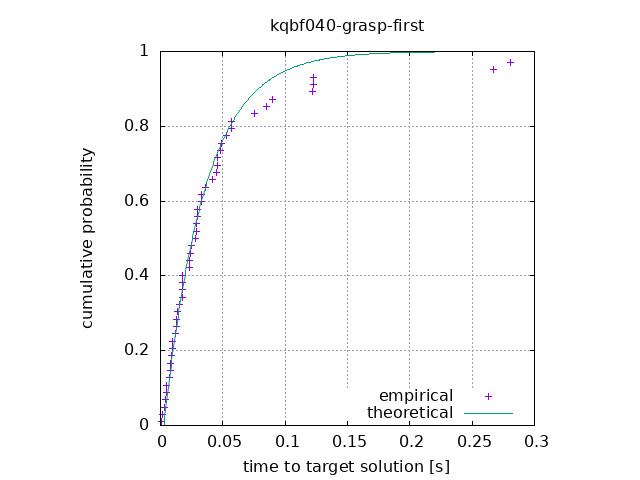
\includegraphics[width=\textwidth]{figure/ttt_plot/kqbf040-grasp-first-exp.jpeg}
        \caption{Cumulative Probability Distribution - Algorithm GRASP First - Problem kqbf040}
        \label{fig:grasp-first-kqbf040-exp}
    \end{subfigure}
    \hfill
    \begin{subfigure}{0.49\textwidth}
        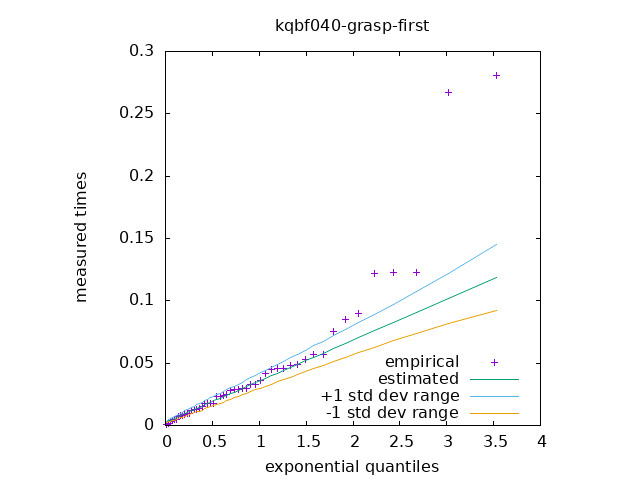
\includegraphics[width=\textwidth]{figure/ttt_plot/kqbf040-grasp-first-qq.jpeg}
        \caption{Q-Q plot - Algorithm GRASP First - Problem kqbf040}
        \label{fig:grasp-first-kqbf040-qq}
    \end{subfigure}
    \caption{Algorithm GRASP First - Problem kqbf040.}
    \label{fig:grasp-first-kqbf040}
\end{figure}


\begin{figure}[H]
    \centering
    \begin{subfigure}{0.49\textwidth}
        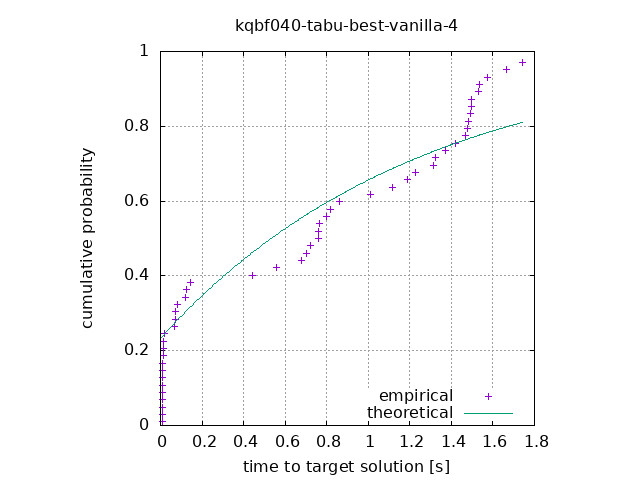
\includegraphics[width=\textwidth]{figure/ttt_plot/kqbf040-tabu-best-vanilla-4-exp.jpeg}
        \caption{Cumulative Probability Distribution - Algorithm Tabu vanilla - Problem kqbf040}
        \label{fig:tabu-vanilla-kqbf040-exp}
    \end{subfigure}
    \hfill
    \begin{subfigure}{0.49\textwidth}
        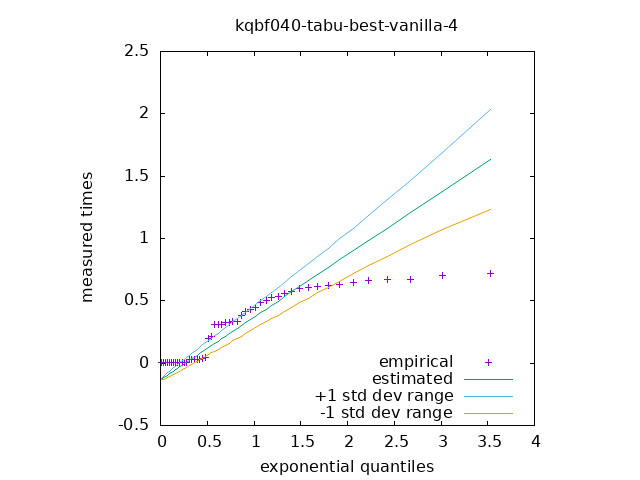
\includegraphics[width=\textwidth]{figure/ttt_plot/kqbf040-tabu-best-vanilla-4-qq.jpeg}
        \caption{Q-Q plot - Algorithm Tabu vanilla - Problem kqbf040}
        \label{fig:tabu-vanilla-kqbf040-qq}
    \end{subfigure}
    \caption{Algorithm Tabu vanilla - Problem kqbf040.}
    \label{fig:tabu-vanilla-kqbf040}
\end{figure}


\begin{figure}[H]
    \centering
    \begin{subfigure}{0.49\textwidth}
        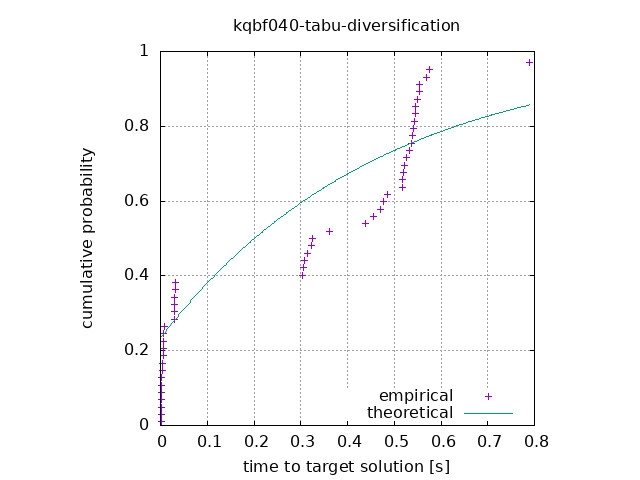
\includegraphics[width=\textwidth]{figure/ttt_plot/kqbf040-tabu-diversification-exp.jpeg}
        \caption{Cumulative Probability Distribution - Algorithm Tabu com Intensificação e Diversificação - Problem kqbf040}
        \label{fig:tabu-com intensificação e diversificação-kqbf040-exp}
    \end{subfigure}
    \hfill
    \begin{subfigure}{0.49\textwidth}
        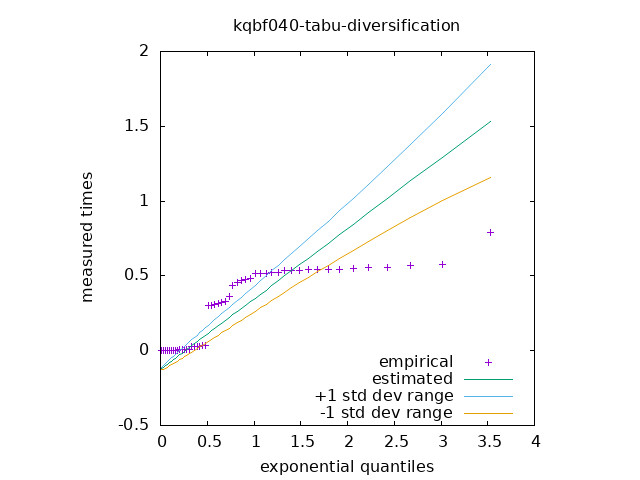
\includegraphics[width=\textwidth]{figure/ttt_plot/kqbf040-tabu-diversification-qq.jpeg}
        \caption{Q-Q plot - Algorithm Tabu com Intensificação e Diversificação - Problem kqbf040}
        \label{fig:tabu-com intensificação e diversificação-kqbf040-qq}
    \end{subfigure}
    \caption{Algorithm Tabu com Intensificação e Diversificação - Problem kqbf040.}
    \label{fig:tabu-com intensificação e diversificação-kqbf040}
\end{figure}


\begin{figure}[H]
    \centering
    \begin{subfigure}{0.49\textwidth}
        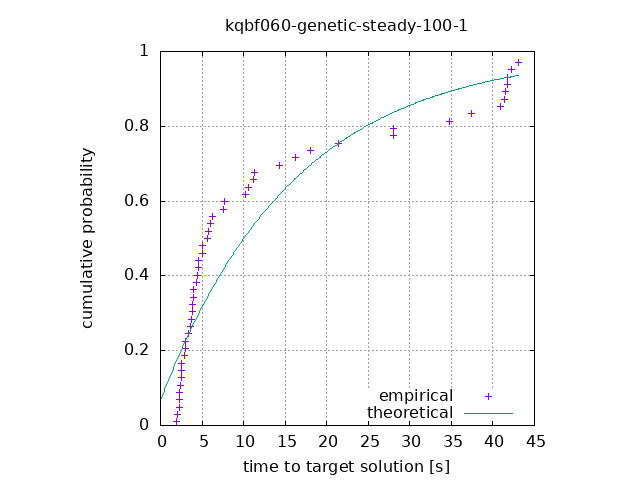
\includegraphics[width=\textwidth]{figure/ttt_plot/kqbf060-genetic-steady-100-1-exp.jpeg}
        \caption{Cumulative Probability Distribution - Algorithm GA steady - Problem kqbf060}
        \label{fig:ga-steady-kqbf060-exp}
    \end{subfigure}
    \hfill
    \begin{subfigure}{0.49\textwidth}
        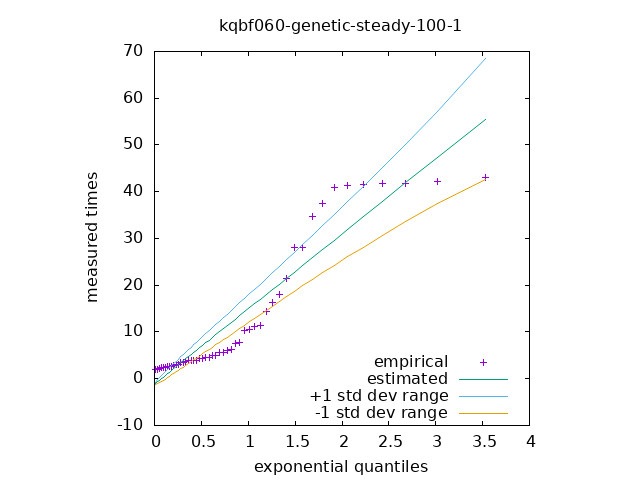
\includegraphics[width=\textwidth]{figure/ttt_plot/kqbf060-genetic-steady-100-1-qq.jpeg}
        \caption{Q-Q plot - Algorithm GA steady - Problem kqbf060}
        \label{fig:ga-steady-kqbf060-qq}
    \end{subfigure}
    \caption{Algorithm GA steady - Problem kqbf060.}
    \label{fig:ga-steady-kqbf060}
\end{figure}


\begin{figure}[H]
    \centering
    \begin{subfigure}{0.49\textwidth}
        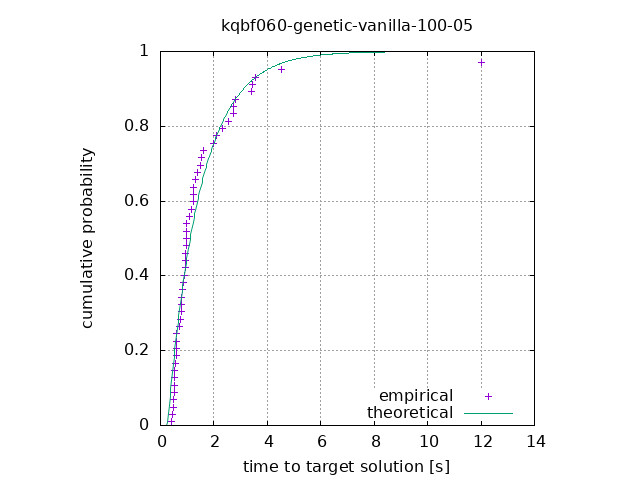
\includegraphics[width=\textwidth]{figure/ttt_plot/kqbf060-genetic-vanilla-100-05-exp.jpeg}
        \caption{Cumulative Probability Distribution - Algorithm GA vanilla - Problem kqbf060}
        \label{fig:ga-vanilla-kqbf060-exp}
    \end{subfigure}
    \hfill
    \begin{subfigure}{0.49\textwidth}
        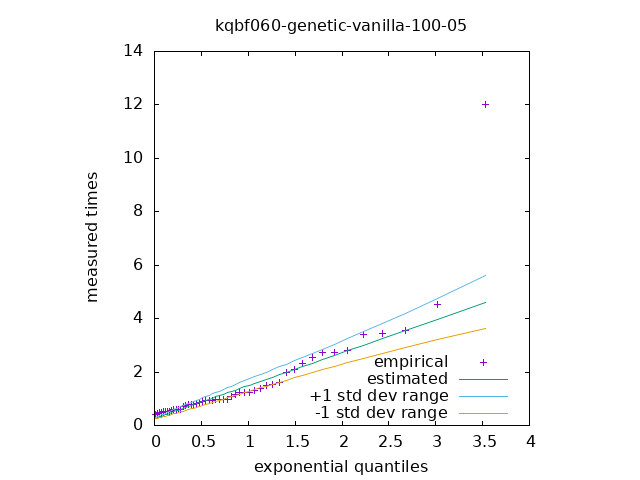
\includegraphics[width=\textwidth]{figure/ttt_plot/kqbf060-genetic-vanilla-100-05-qq.jpeg}
        \caption{Q-Q plot - Algorithm GA vanilla - Problem kqbf060}
        \label{fig:ga-vanilla-kqbf060-qq}
    \end{subfigure}
    \caption{Algorithm GA vanilla - Problem kqbf060.}
    \label{fig:ga-vanilla-kqbf060}
\end{figure}


\begin{figure}[H]
    \centering
    \begin{subfigure}{0.49\textwidth}
        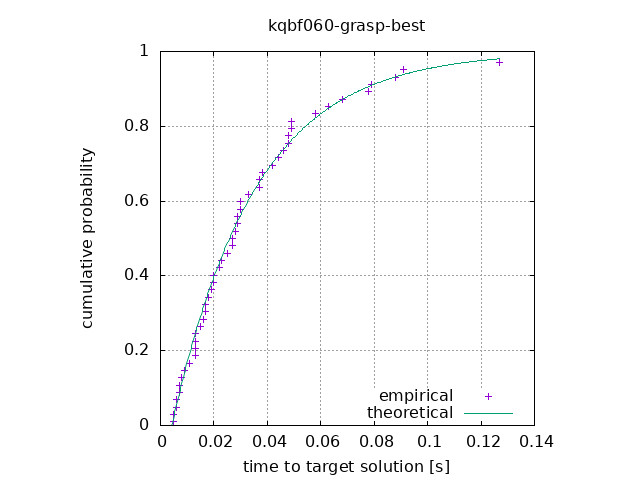
\includegraphics[width=\textwidth]{figure/ttt_plot/kqbf060-grasp-best-exp.jpeg}
        \caption{Cumulative Probability Distribution - Algorithm GRASP Best - Problem kqbf060}
        \label{fig:grasp-best-kqbf060-exp}
    \end{subfigure}
    \hfill
    \begin{subfigure}{0.49\textwidth}
        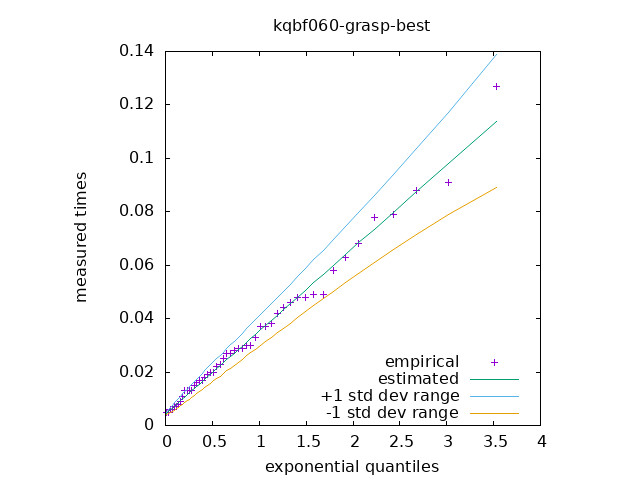
\includegraphics[width=\textwidth]{figure/ttt_plot/kqbf060-grasp-best-qq.jpeg}
        \caption{Q-Q plot - Algorithm GRASP Best - Problem kqbf060}
        \label{fig:grasp-best-kqbf060-qq}
    \end{subfigure}
    \caption{Algorithm GRASP Best - Problem kqbf060.}
    \label{fig:grasp-best-kqbf060}
\end{figure}


\begin{figure}[H]
    \centering
    \begin{subfigure}{0.49\textwidth}
        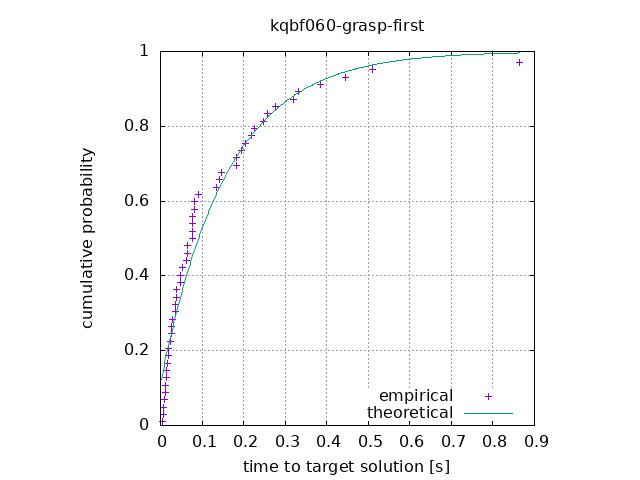
\includegraphics[width=\textwidth]{figure/ttt_plot/kqbf060-grasp-first-exp.jpeg}
        \caption{Cumulative Probability Distribution - Algorithm GRASP First - Problem kqbf060}
        \label{fig:grasp-first-kqbf060-exp}
    \end{subfigure}
    \hfill
    \begin{subfigure}{0.49\textwidth}
        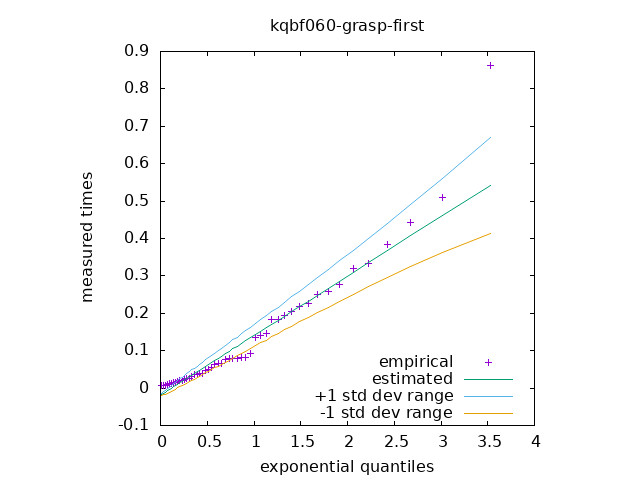
\includegraphics[width=\textwidth]{figure/ttt_plot/kqbf060-grasp-first-qq.jpeg}
        \caption{Q-Q plot - Algorithm GRASP First - Problem kqbf060}
        \label{fig:grasp-first-kqbf060-qq}
    \end{subfigure}
    \caption{Algorithm GRASP First - Problem kqbf060.}
    \label{fig:grasp-first-kqbf060}
\end{figure}


\begin{figure}[H]
    \centering
    \begin{subfigure}{0.49\textwidth}
        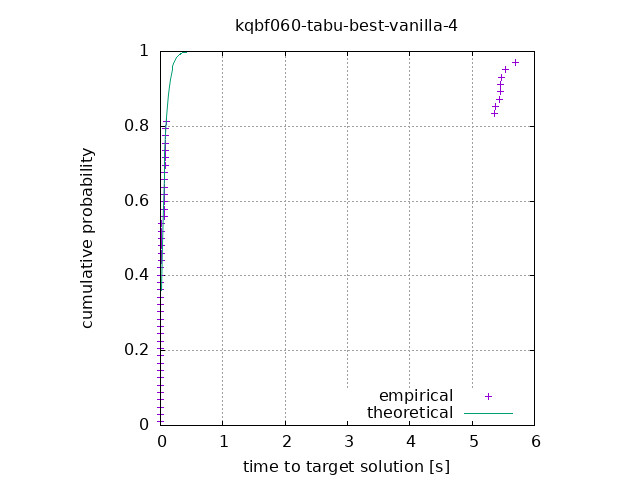
\includegraphics[width=\textwidth]{figure/ttt_plot/kqbf060-tabu-best-vanilla-4-exp.jpeg}
        \caption{Cumulative Probability Distribution - Algorithm Tabu vanilla - Problem kqbf060}
        \label{fig:tabu-vanilla-kqbf060-exp}
    \end{subfigure}
    \hfill
    \begin{subfigure}{0.49\textwidth}
        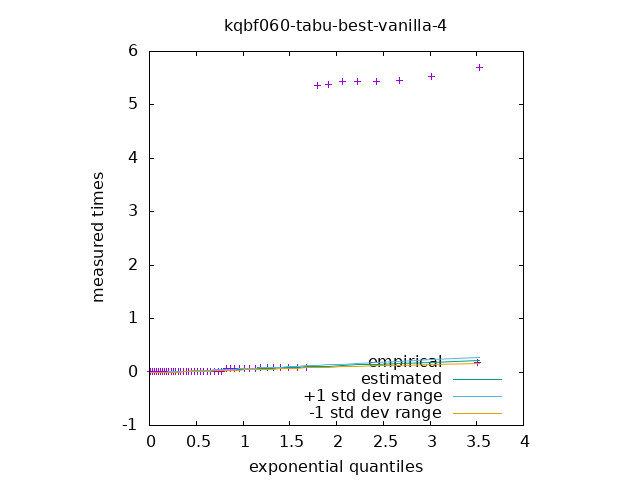
\includegraphics[width=\textwidth]{figure/ttt_plot/kqbf060-tabu-best-vanilla-4-qq.jpeg}
        \caption{Q-Q plot - Algorithm Tabu vanilla - Problem kqbf060}
        \label{fig:tabu-vanilla-kqbf060-qq}
    \end{subfigure}
    \caption{Algorithm Tabu vanilla - Problem kqbf060.}
    \label{fig:tabu-vanilla-kqbf060}
\end{figure}


\begin{figure}[H]
    \centering
    \begin{subfigure}{0.49\textwidth}
        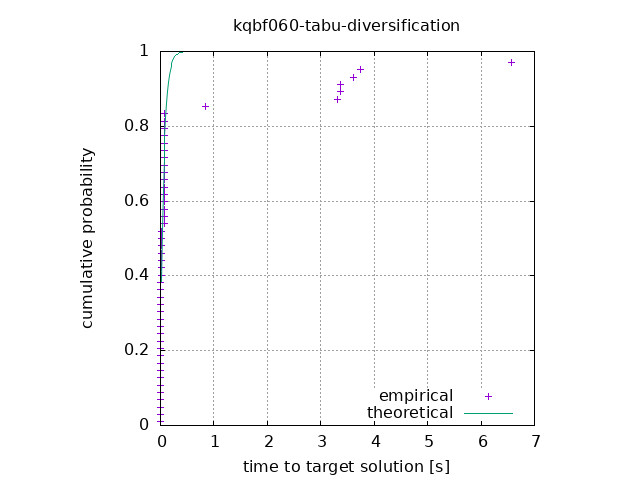
\includegraphics[width=\textwidth]{figure/ttt_plot/kqbf060-tabu-diversification-exp.jpeg}
        \caption{Cumulative Probability Distribution - Algorithm Tabu com Intensificação e Diversificação - Problem kqbf060}
        \label{fig:tabu-com intensificação e diversificação-kqbf060-exp}
    \end{subfigure}
    \hfill
    \begin{subfigure}{0.49\textwidth}
        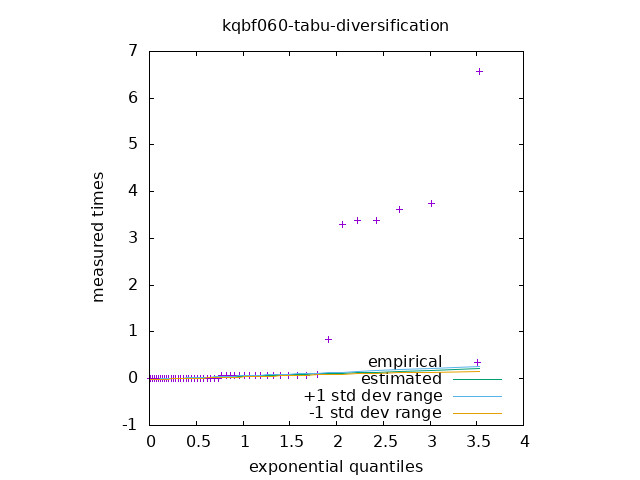
\includegraphics[width=\textwidth]{figure/ttt_plot/kqbf060-tabu-diversification-qq.jpeg}
        \caption{Q-Q plot - Algorithm Tabu com Intensificação e Diversificação - Problem kqbf060}
        \label{fig:tabu-com intensificação e diversificação-kqbf060-qq}
    \end{subfigure}
    \caption{Algorithm Tabu com Intensificação e Diversificação - Problem kqbf060.}
    \label{fig:tabu-com intensificação e diversificação-kqbf060}
\end{figure}


\begin{figure}[H]
    \centering
    \begin{subfigure}{0.49\textwidth}
        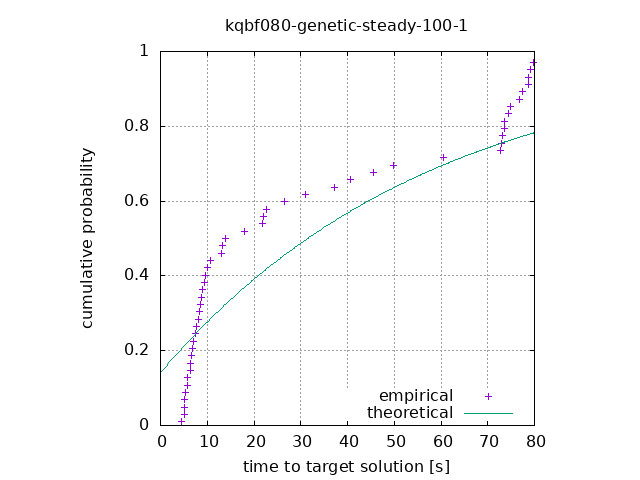
\includegraphics[width=\textwidth]{figure/ttt_plot/kqbf080-genetic-steady-100-1-exp.jpeg}
        \caption{Cumulative Probability Distribution - Algorithm GA steady - Problem kqbf080}
        \label{fig:ga-steady-kqbf080-exp}
    \end{subfigure}
    \hfill
    \begin{subfigure}{0.49\textwidth}
        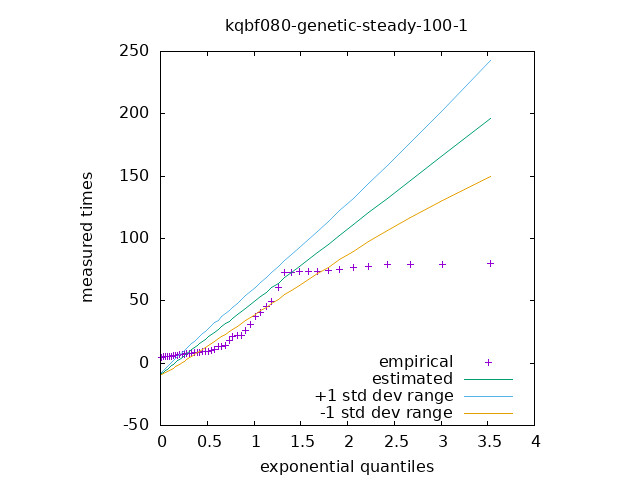
\includegraphics[width=\textwidth]{figure/ttt_plot/kqbf080-genetic-steady-100-1-qq.jpeg}
        \caption{Q-Q plot - Algorithm GA steady - Problem kqbf080}
        \label{fig:ga-steady-kqbf080-qq}
    \end{subfigure}
    \caption{Algorithm GA steady - Problem kqbf080.}
    \label{fig:ga-steady-kqbf080}
\end{figure}


\begin{figure}[H]
    \centering
    \begin{subfigure}{0.49\textwidth}
        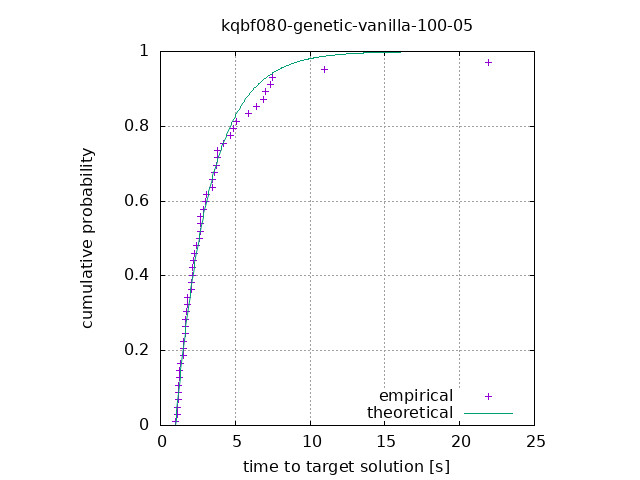
\includegraphics[width=\textwidth]{figure/ttt_plot/kqbf080-genetic-vanilla-100-05-exp.jpeg}
        \caption{Cumulative Probability Distribution - Algorithm GA vanilla - Problem kqbf080}
        \label{fig:ga-vanilla-kqbf080-exp}
    \end{subfigure}
    \hfill
    \begin{subfigure}{0.49\textwidth}
        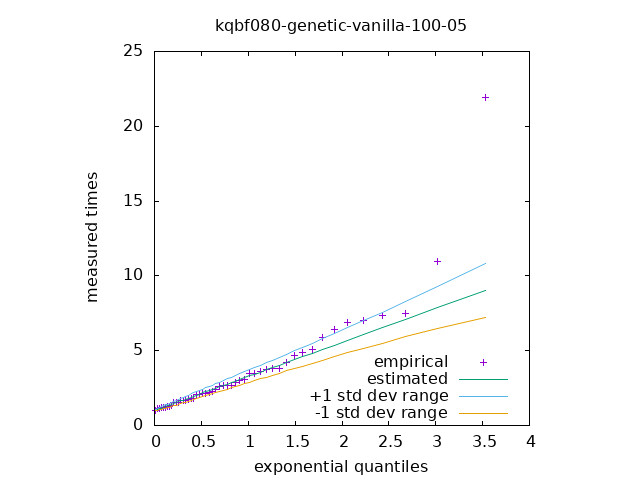
\includegraphics[width=\textwidth]{figure/ttt_plot/kqbf080-genetic-vanilla-100-05-qq.jpeg}
        \caption{Q-Q plot - Algorithm GA vanilla - Problem kqbf080}
        \label{fig:ga-vanilla-kqbf080-qq}
    \end{subfigure}
    \caption{Algorithm GA vanilla - Problem kqbf080.}
    \label{fig:ga-vanilla-kqbf080}
\end{figure}


\begin{figure}[H]
    \centering
    \begin{subfigure}{0.49\textwidth}
        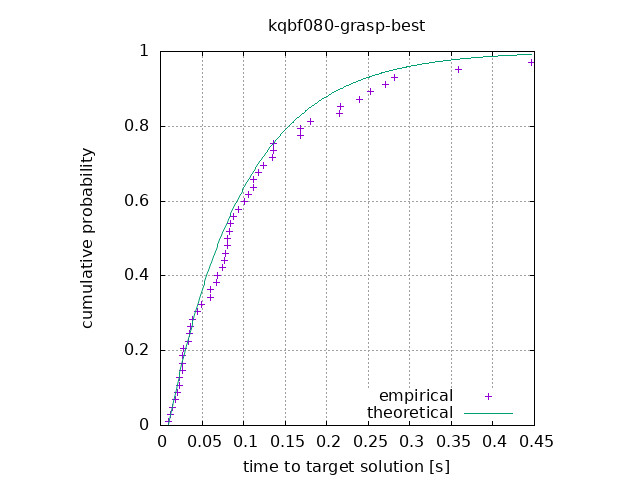
\includegraphics[width=\textwidth]{figure/ttt_plot/kqbf080-grasp-best-exp.jpeg}
        \caption{Cumulative Probability Distribution - Algorithm GRASP Best - Problem kqbf080}
        \label{fig:grasp-best-kqbf080-exp}
    \end{subfigure}
    \hfill
    \begin{subfigure}{0.49\textwidth}
        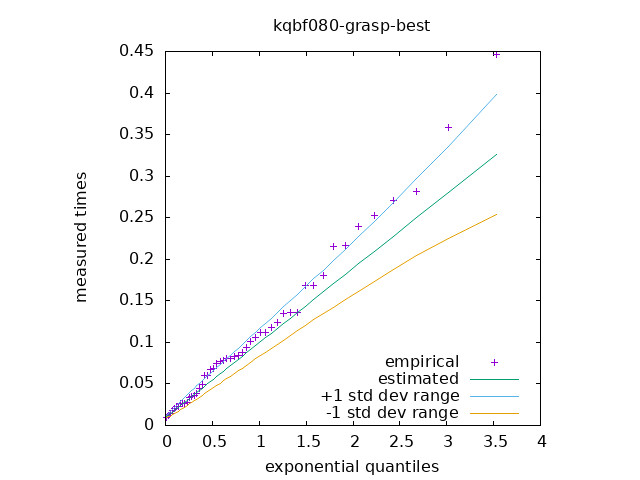
\includegraphics[width=\textwidth]{figure/ttt_plot/kqbf080-grasp-best-qq.jpeg}
        \caption{Q-Q plot - Algorithm GRASP Best - Problem kqbf080}
        \label{fig:grasp-best-kqbf080-qq}
    \end{subfigure}
    \caption{Algorithm GRASP Best - Problem kqbf080.}
    \label{fig:grasp-best-kqbf080}
\end{figure}


\begin{figure}[H]
    \centering
    \begin{subfigure}{0.49\textwidth}
        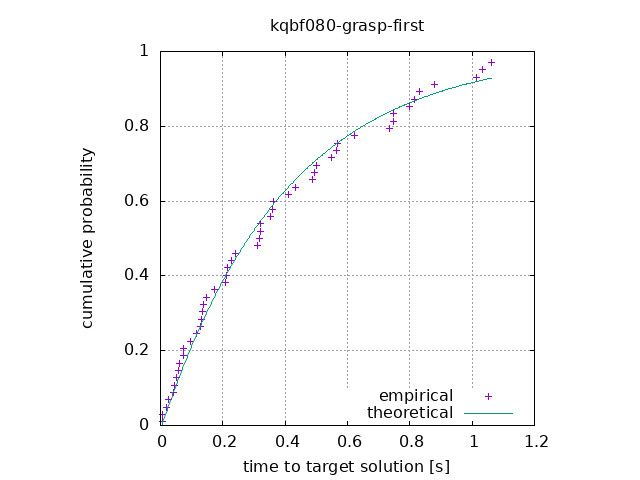
\includegraphics[width=\textwidth]{figure/ttt_plot/kqbf080-grasp-first-exp.jpeg}
        \caption{Cumulative Probability Distribution - Algorithm GRASP First - Problem kqbf080}
        \label{fig:grasp-first-kqbf080-exp}
    \end{subfigure}
    \hfill
    \begin{subfigure}{0.49\textwidth}
        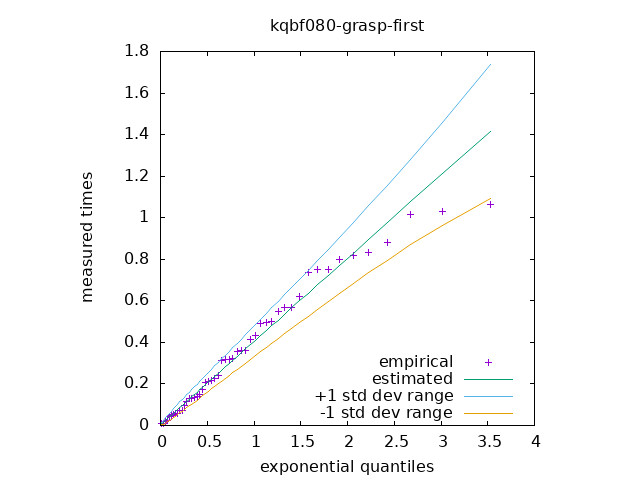
\includegraphics[width=\textwidth]{figure/ttt_plot/kqbf080-grasp-first-qq.jpeg}
        \caption{Q-Q plot - Algorithm GRASP First - Problem kqbf080}
        \label{fig:grasp-first-kqbf080-qq}
    \end{subfigure}
    \caption{Algorithm GRASP First - Problem kqbf080.}
    \label{fig:grasp-first-kqbf080}
\end{figure}


\begin{figure}[H]
    \centering
    \begin{subfigure}{0.49\textwidth}
        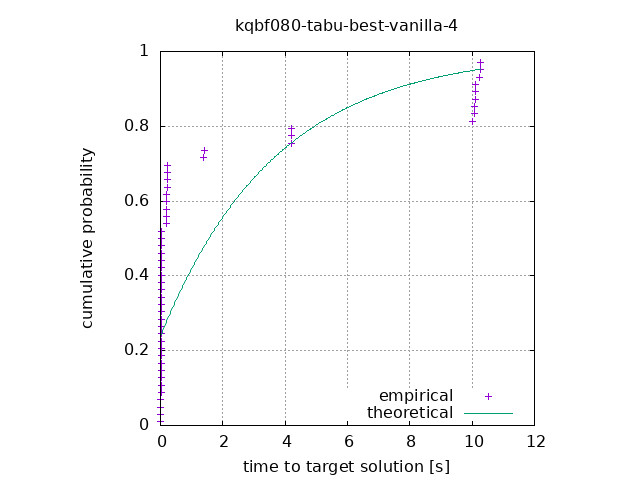
\includegraphics[width=\textwidth]{figure/ttt_plot/kqbf080-tabu-best-vanilla-4-exp.jpeg}
        \caption{Cumulative Probability Distribution - Algorithm Tabu vanilla - Problem kqbf080}
        \label{fig:tabu-vanilla-kqbf080-exp}
    \end{subfigure}
    \hfill
    \begin{subfigure}{0.49\textwidth}
        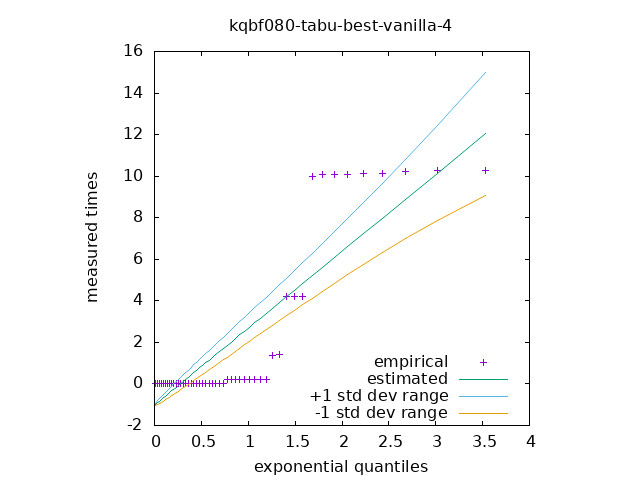
\includegraphics[width=\textwidth]{figure/ttt_plot/kqbf080-tabu-best-vanilla-4-qq.jpeg}
        \caption{Q-Q plot - Algorithm Tabu vanilla - Problem kqbf080}
        \label{fig:tabu-vanilla-kqbf080-qq}
    \end{subfigure}
    \caption{Algorithm Tabu vanilla - Problem kqbf080.}
    \label{fig:tabu-vanilla-kqbf080}
\end{figure}


\begin{figure}[H]
    \centering
    \begin{subfigure}{0.49\textwidth}
        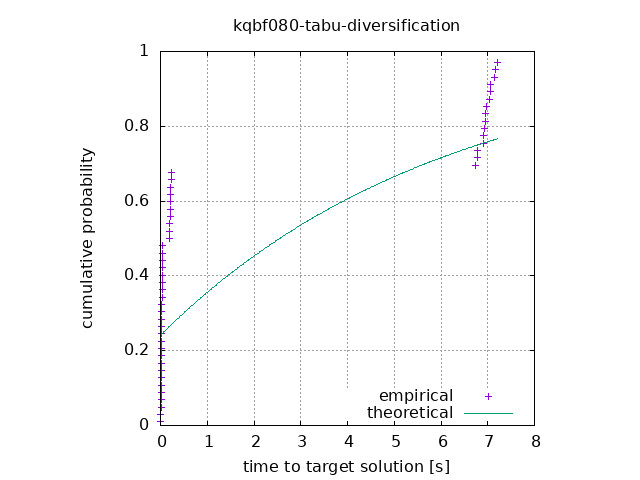
\includegraphics[width=\textwidth]{figure/ttt_plot/kqbf080-tabu-diversification-exp.jpeg}
        \caption{Cumulative Probability Distribution - Algorithm Tabu com Intensificação e Diversificação - Problem kqbf080}
        \label{fig:tabu-com intensificação e diversificação-kqbf080-exp}
    \end{subfigure}
    \hfill
    \begin{subfigure}{0.49\textwidth}
        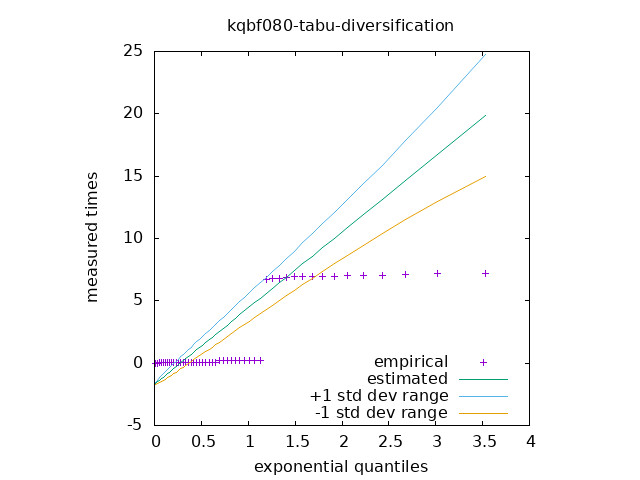
\includegraphics[width=\textwidth]{figure/ttt_plot/kqbf080-tabu-diversification-qq.jpeg}
        \caption{Q-Q plot - Algorithm Tabu com Intensificação e Diversificação - Problem kqbf080}
        \label{fig:tabu-com intensificação e diversificação-kqbf080-qq}
    \end{subfigure}
    \caption{Algorithm Tabu com Intensificação e Diversificação - Problem kqbf080.}
    \label{fig:tabu-com intensificação e diversificação-kqbf080}
\end{figure}
